
\sloppy
\begin{center}{\fontsize{16pt}{16pt}\selectfont \textbf{Python Date  $  \&  $ Time} \\}\end{center} \par

 \section{Python Date and Time}
\noindent 
 Program Python dapat menangani tanggal dan waktu dengan beberapa cara. Mengkonversi antara format tanggal adalah tugas umum untuk komputer. Waktu dan modul kalender Python membantu melacak tanggal dan waktu. \par

\noindent 
\begin{itemize}
	\item What is Tick?
\end{itemize}
\noindent 
Selang waktu adalah bilangan floating-point dalam satuan detik. Instansi tertentu dalam waktu dinyatakan dalam hitungan detik sejak pukul 12:00 pagi, 1 Januari 1970 (epoch). \par
\noindent 
Ada modul waktu populer yang tersedia dengan Python yang menyediakan fungsi untuk bekerja dengan waktu, dan untuk mengkonversi antara representasi. Fungsi time.time () mengembalikan waktu sistem saat ini di kutu sejak pukul 12:00, 1 Januari 1970 (zaman). \par
\vspace{12pt}
\vspace{\baselineskip}
\noindent 
\begin{verbatim}
Example 
#!/usr/bin/python
import~time;#This is required to include time module.
ticks = time.time() 
print "Number of ticks since 
12:00am, January 1, 1970:", ticks \par 
\end{verbatim}
\vspace{10pt}
Hal ini akan menghasilkan sesuatu sebagai berikut - \par
\noindent 
Number of ticks since 12:00am, January 1, 1970: 7186862.73399 \par
\vspace{\baselineskip}
\noindent 
Tanggal aritmatika mudah dilakukan dengan kutu. Namun, tanggal sebelum zaman tidak dapat diwakili dalam formulir ini. Tanggal di masa depan juga tidak dapat diwakili dengan cara ini - titik potong adalah sekitar 2038 untuk UNIX dan Windows. \par
\vspace{\baselineskip}
\noindent 
\begin{itemize}
	\item What is TimeTuple?
\end{itemize}
\noindent 
Banyak fungsi waktu Python menangani waktu sebagai tuple dari 9 nomor, seperti yang ditunjukkan di bawah ini – \par
\vspace{12pt}
\noindent 
Tuple di atas setara dengan struct $  \_  $time structure. Struktur ini memiliki atribut berikut – \par
\vspace{12pt}
\noindent 
\begin{enumerate}
	\item Getting current time
\end{enumerate}
\noindent 
Untuk menerjemahkan waktu instan dari satu detik sejak nilai floating-point ke waktu tupel, lewati nilai floating-point ke fungsi (mis., Localtime) yang mengembalikan waktu tupel dengan semua sembilan item valid. \par
 
 \begin{verbatim}
#!/usr/bin/python
import time; 
localtime = time.localtime(time.time()) \par
print "Local current time :", localtime \par
 \end{verbatim}
Ini akan menghasilkan hasil berikut, yang dapat diformat dalam bentuk lain yang sesuai - \par
\noindent 
Local current time : time.struct $  \_  $time(tm $  \_  $year=2013, tm $  \_  $mon=7,  \par
\noindent 
tm $  \_  $mday=17, tm $  \_  $hour=21, tm $  \_  $min=26, tm $  \_  $sec=3, tm $  \_  $wday=2, tm $  \_  $yday=198, tm $  \_  $isdst=0) \par
\vspace{12pt}
\vspace{12pt}
\vspace{12pt}
\vspace{12pt}
\vspace{12pt}
\vspace{12pt}
\vspace{12pt}
\vspace{12pt}

\begin{itemize}
	\item Support Opperation
\end{itemize}

\begin{figure}[ht]
	\centerline{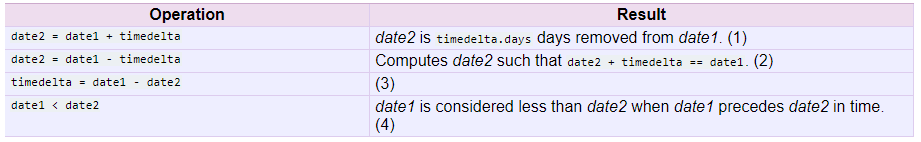
\includegraphics[width=0.90\textwidth]{figures/DateTime2}}
	\caption{Support Operation}
	\label{Support Opperation}
\end{figure}

\vspace{\baselineskip}
\noindent 
\begin{enumerate}
	\item Getting formatted time \par
\end{enumerate}
\noindent 
Anda dapat memformat kapan saja sesuai kebutuhan Anda, namun metode sederhana untuk mendapatkan waktu dalam format yang mudah dibaca adalah asctime () - \par
\noindent 
 \hspace*{0.5in}  $  \#  $!/usr/bin/python \par
\noindent 
 \hspace*{0.5in} import time; \par
\vspace{12pt}
\noindent 
 \hspace*{0.5in} localtime = time.asctime( time.localtime(time.time()) ) \par
\noindent 
 \hspace*{0.5in} print "Local current time :", localtime \par
\vspace{12pt}
\noindent 
Ini akan menghasilkan hasil sebagai berikut - \par
\noindent 
 \hspace*{0.5in} Local current time : Tue Jan 13 10:17:09 2009 \par
\vspace{12pt}
\vspace{12pt}
\noindent 
public static String getCurrentTimeStamp ()  $  \{  $ \par
\noindent 
 $  $ $  $ $  $ $  $ SimpleDateFormat sdfDate = new SimpleDateFormat ("yyyy-MM-dd HH: mm: ss"); // dd / MM / yyyy \par
\noindent 
 $  $ $  $ $  $ $  $ Tanggal sekarang = tanggal baru (); \par
\noindent 
 $  $ $  $ $  $ $  $ String strDate = sdfDate.format (sekarang); \par
\noindent 
 $  $ $  $ $  $ $  $ kembali strDate; \par
\noindent 
 $  \}  $ \par
\vspace{\baselineskip}
\noindent 
Saya mendapatkan tanggal dalam format 2009-09-22 16:47:08 (YYYY-MM-DD HH: MI: Sec). \par
\vspace{12pt}
\noindent 
Tapi saya ingin mengambil waktu sekarang dalam format 2009-09-22 16: 47: 08.128 ((YYYY-MM-DD HH: MI: Sec.Ms). \par
\vspace{12pt}
\noindent 
dimana 128 menceritakan milidetik. \par
\vspace{12pt}
\noindent 
SimpleTextFormat akan bekerja dengan baik. Di sini satuan waktu paling rendah adalah yang kedua, tapi bagaimana cara mendapatkan milidetik juga? \par
\noindent 
FYI, kelas tanggal tua yang merepotkan seperti java.util.Date, java.util.Calendar, dan java.text.SimpleTextFormat sekarang warisan, digantikan oleh kelas java.time. \par
\vspace{12pt}
\vspace{14pt}

\begin{itemize}
	\item Instance Attributes
\end{itemize}

\begin{figure}[ht]
	\centerline{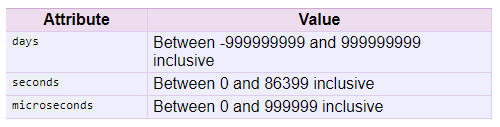
\includegraphics[width=0.90\textwidth]{figures/DateTime}}
	\caption{Instance Attributes}
	\label{Instance Attributes}
\end{figure}


\vspace{\baselineskip}
\noindent 
\begin{enumerate}
	\item Getting calendar for a month
\end{enumerate}
\noindent 
Modul kalender memberikan berbagai macam metode untuk dimainkan dengan kalender tahunan dan bulanan. Di sini, kami mencetak kalender untuk bulan tertentu (Jan 2008) - \par
\noindent 
 \hspace*{0.5in}  $  \#  $!/usr/bin/python \par
\noindent 
 \hspace*{0.5in} import calendar \par
\vspace{12pt}
\noindent 
 \hspace*{0.5in} cal = calendar.month(2008, 1) \par
\noindent 
 \hspace*{0.5in} print "Here is the calendar:" \par
\noindent 
 \hspace*{0.5in} print cal \par
\vspace{\baselineskip}
\noindent 
Ini akan menghasilkan hasil sebagai berikut - \par
\noindent 
 \hspace*{0.5in} Here is the calendar: \par
\noindent 
~~~  \hspace*{0.5in}  \hspace*{0.5in} January 2008 \par
\noindent 
 \hspace*{0.5in} Mo Tu We Th Fr Sa Su \par
\noindent 
~~~  \hspace*{0.5in}  \hspace*{0.5in} 1~ 2~~3~~4  5  6 \par
\noindent 
  \hspace*{0.5in}  \hspace*{0.5in} 7~ 8~ 9 10 11 12 13 \par
\noindent 
 \hspace*{0.5in}  \hspace*{0.5in} 14 15 16 17 18 19 20 \par
\noindent 
 \hspace*{0.5in}  \hspace*{0.5in} 21 22 23 24 25 26 27 \par
\noindent 
 \hspace*{0.5in}  \hspace*{0.5in} 28 29 30 31 \par
\noindent 

 \subsection {Android}
 \vspace{\baselineskip}
\noindent 
Pergi ke hari tertentu \par
\noindent 
Buka Google Kalender app Calendar. \par
\noindent 
Di kiri atas, ketuk nama bulan. Misalnya, January Down Arrow. \par
\noindent 
Gesek ke kiri atau kanan untuk pergi ke bulan lainnya. \par
\noindent 
Ketuk tanggal untuk melihat acara pada hari itu. \par
\noindent 
Kembali ke hari ini: Di pojok kanan atas, sentuh View today Event. \par
\vspace{12pt}
\noindent 
Pilih berapa hari untuk melihat \par
\noindent 
Saat membuka aplikasi Kalender, Anda akan melihat daftar acara mendatang Anda. Anda dapat mengalihkan pandangan untuk melihat keseluruhan hari atau beberapa hari Anda. \par
\vspace{12pt}
\noindent 
Buka Google Kalender app Calendar. \par
\noindent 
Di sudut kiri atas, tekan Menu Menu. \par
\noindent 
Pilih tampilan, seperti Jadwal atau Bulan. Untuk melihat semua acara, sasaran, dan pengingat Anda dalam daftar yang dipecah berdasarkan hari, pilih "Jadwal". \par
\noindent 

 \subsection {Computer}
\noindent 
Ubah tampilan kalender Anda \par
\noindent 
Ubah sementara \par
\noindent 
Tetapkan tampilan default baru \par
\noindent 
Arahkan kalender Anda \par
\noindent 
Ada dua cara untuk berpindah antar tanggal: \par
\vspace{12pt}
\noindent 
Gunakan tanda panah di pojok kiri atas Kalender untuk beralih ke tanggal terakhir di masa lalu atau masa depan. \par
\noindent 
Gunakan kalender kecil di pojok kiri atas untuk memilih tanggal. \par
\noindent 
Untuk kembali ke tanggal hari ini, klik Hari ini di pojok kiri atas. \par
\vspace{12pt}
\noindent 
Artikel terkait \par
\noindent 
Ubah pengaturan kalender Anda \par
\noindent 
Buat kalender baru \par


\noindent 
 \subsection { Iphone dan Ipad }
\noindent 
Pergi ke hari tertentu \par
\noindent 
Buka Google Kalender app Calendar. \par
\noindent 
Di kiri atas, ketuk nama bulan. Misalnya, January Down Arrow. \par
\noindent 
Gesek ke kiri atau kanan untuk pergi ke bulan lainnya. \par
\noindent 
Ketuk tanggal untuk melihat acara pada hari itu. \par
\noindent 
Kembali ke hari ini: Di pojok kanan atas, sentuh View today Event. \par
\vspace{12pt}
\noindent 
Pilih berapa hari untuk melihat \par
\noindent 
Saat membuka aplikasi Kalender, Anda akan melihat daftar acara mendatang Anda. Anda dapat mengalihkan pandangan untuk melihat keseluruhan hari atau beberapa hari Anda. \par
\vspace{12pt}
\noindent 
Buka Google Kalender app Calendar. \par
\noindent 
Di sudut kiri atas, tekan Menu Menu. \par
\noindent 
Pilih tampilan, seperti Jadwal atau Bulan. Untuk melihat semua acara, sasaran, dan pengingat Anda dalam daftar yang dipecah berdasarkan hari, pilih "Jadwal". \par
\noindent 
Ubah pengaturan Anda \par
\noindent 
Pelajari cara mengubah setelan kalender Anda, termasuk tampilan kalender dan hari dimulai. \par
\vspace{\baselineskip}
\noindent 
\begin{itemize}
\item The time Module
\end{itemize}
\noindent 
 \hspace*{0.5in} Ada modul waktu populer yang tersedia dengan Python yang menyediakan fungsi untuk bekerja dengan waktu dan untuk mengkonversi antara representasi. Berikut adalah daftar semua metode yang tersedia – \par
\noindent 
Modul ini menyediakan berbagai fungsi yang berkaitan dengan waktu. Untuk fungsionalitas terkait, lihat juga modul kalender dan kalender. \par
\vspace{12pt}
\noindent 
Meski modul ini selalu tersedia, tidak semua fungsi tersedia di semua platform. Sebagian besar fungsi yang didefinisikan dalam modul ini memanggil fungsi library C library dengan nama yang sama. Terkadang ada baiknya untuk berkonsultasi dengan dokumentasi platform, karena semantik fungsi ini bervariasi antar platform. \par
\noindent 
Penjelasan tentang beberapa terminologi dan konvensi adalah teratur. \par
\vspace{12pt}
\noindent 
Epoch adalah titik di mana waktu dimulai. Pada tanggal 1 Januari tahun itu, pada 0 jam, "waktu sejak zaman" adalah nol. Untuk Unix, eposnya adalah 1970. Untuk mengetahui apa zamannya, lihatlah gmtime (0). \par
\vspace{12pt}
\noindent 
Fungsi dalam modul ini tidak menangani tanggal dan waktu sebelum zaman atau jauh di masa depan. Titik potong di masa depan ditentukan oleh perpustakaan C; untuk Unix, biasanya pada tahun 2038. \par
\vspace{12pt}
\noindent 
Masalah tahun 2000 (Y2K): Python bergantung pada perpustakaan C platform, yang umumnya tidak memiliki masalah tahun 2000, karena semua tanggal dan waktu diwakili secara internal sebagai detik sejak zaman itu. Fungsi menerima struct $  \_  $time (lihat di bawah) umumnya memerlukan 4 digit tahun. Untuk kompatibilitas, 2 digit tahun didukung jika variabel modul accept2dyear adalah bilangan bulat nol nol; variabel ini diinisialisasi ke 1 kecuali variabel lingkungan PYTHONY2K diatur ke string yang tidak kosong, dalam hal ini diinisialisasi menjadi 0. Dengan demikian, Anda dapat mengatur PYTHONY2K ke string yang tidak kosong di lingkungan untuk meminta digit 4 digit untuk semua masukan tahun. Bila 2 digit tahun diterima, mereka dikonversi sesuai dengan standar POSIX atau X / Open: nilai 69-99 dipetakan ke 1969-1999, dan nilai 0-68 dipetakan ke 2000-2068. Nilai 100-1899 selalu ilegal. \par
\vspace{12pt}
\noindent 
UTC adalah Coordinated Universal Time (sebelumnya dikenal sebagai Greenwich Mean Time, atau GMT). Akronim UTC bukan kesalahan tapi kompromi antara bahasa Inggris dan Prancis. \par
\vspace{12pt}
\noindent 
DST adalah Daylight Saving Time, penyesuaian zona waktu dengan (biasanya) satu jam selama bagian tahun ini. Aturan DST adalah sihir (ditentukan oleh hukum setempat) dan bisa berubah dari tahun ke tahun. Perpustakaan C memiliki tabel yang berisi peraturan lokal (seringkali dibaca dari file sistem untuk fleksibilitas) dan merupakan satu-satunya sumber Kebijaksanaan Sejati dalam hal ini. \par
\vspace{12pt}
\noindent 
Ketepatan berbagai fungsi real-time mungkin kurang dari yang disarankan oleh unit di mana nilai atau argumen mereka diungkapkan. Misalnya. Pada sebagian besar sistem Unix, jam "kutu" hanya 50 atau 100 kali per detik. \par
\vspace{12pt}
\noindent 
Di sisi lain, ketepatan waktu () dan sleep () lebih baik daripada padanan Unix mereka: waktu dinyatakan sebagai bilangan floating point, waktu () mengembalikan waktu paling akurat yang tersedia (menggunakan Unix gettimeofday () jika tersedia), dan tidur () akan menerima waktu dengan pecahan tak-nol (Unix select () digunakan untuk menerapkan ini, jika tersedia). \par
\vspace{12pt}
\noindent 
Nilai waktu seperti yang dikembalikan oleh gmtime (), localtime (), dan strptime (), dan diterima oleh asctime (), mktime () dan strftime (), dapat dianggap sebagai urutan dari 9 bilangan bulat. Nilai kembalian gmtime (), localtime (), dan strptime () juga menawarkan nama atribut untuk masing-masing bidang. \par
\vspace{12pt}
\noindent 
Lihat struct $  \_  $time untuk deskripsi objek ini. \par
\vspace{12pt}
\noindent 
Berubah dalam versi 2.2: Urutan nilai waktu diubah dari tupel menjadi struct $  \_  $time, dengan penambahan nama atribut untuk field. \par
\vspace{\baselineskip}
\noindent 
\begin{itemize}
\item The calendar Module
\end{itemize}
\noindent 
Modul kalender memasok fungsi yang berhubungan dengan kalender, termasuk fungsi untuk mencetak kalender teks untuk bulan atau tahun tertentu. \par
\noindent 
Secara default, kalender mengambil hari Senin sebagai hari pertama minggu dan minggu sebagai yang terakhir. Untuk mengubah ini, fungsi call calendar.setfirstweekday (). \par
\noindent 
Berikut adalah daftar fungsi yang tersedia dengan modul kalender: \par
\noindent 
Modul ini memungkinkan Anda untuk menampilkan kalender seperti program cal Unix, dan menyediakan fungsi berguna tambahan yang terkait dengan kalender. Secara default, kalender ini Senin sebagai hari pertama dalam seminggu, dan hari minggu sebagai yang terakhir (konvensi Eropa). Gunakan setfirstweekday () untuk mengatur hari pertama dalam seminggu sampai Minggu (6) atau ke hari kerja lainnya. Parameter yang menentukan tanggal diberikan sebagai bilangan bulat. Untuk fungsionalitas terkait, lihat juga modul waktu dan waktu. \par
\vspace{12pt}
\noindent 
Sebagian besar fungsi dan kelas bergantung pada modul datetime yang menggunakan kalender ideal, kalender Gregorian saat ini tanpa batas diperpanjang di kedua arah. Ini sesuai dengan definisi kalender "pakar Gregorian" di buku Dershowitz dan Reingold "Perhitungan Calendrical", di mana kalender dasar untuk semua perhitungan. \par
\vspace{12pt}
\noindent 
kalender kelas.Calendar ([firstweekday]) \par
\noindent 
Membuat objek Kalender. Firstweekday adalah bilangan bulat yang menentukan hari pertama dalam seminggu. 0 adalah hari Senin (default), 6 adalah hari minggu. \par
\vspace{12pt}
\noindent 
Objek Kalender menyediakan beberapa metode yang dapat digunakan untuk menyiapkan data kalender untuk pemformatan. Kelas ini tidak melakukan format apapun itu sendiri. Ini adalah tugas dari subclass. \par
\vspace{12pt}
\noindent 
Baru di versi 2.5. \par
\vspace{12pt}
\noindent 
Contoh kalender memiliki metode berikut: \par
\vspace{12pt}
\noindent 
iterweekdays () \par
\noindent 
Kembalikan iterator untuk nomor hari minggu yang akan digunakan selama satu minggu. Nilai pertama dari iterator akan sama dengan nilai properti first weekekday. \par
\vspace{12pt}
\noindent 
ini bulan depan (tahun, bulan) \par
\noindent 
Kembalikan iterator untuk bulan bulan (1-12) di tahun tahun. Iterator ini akan mengembalikan semua hari (sebagai objek datetime.date) untuk bulan dan semua hari sebelum awal bulan atau setelah akhir bulan yang diperlukan untuk mendapatkan minggu yang lengkap. \par
\vspace{12pt}
\noindent 
itermonthdays2 (tahun, bulan) \par
\noindent 
Kembalikan iterator untuk bulan bulan di tahun yang sama dengan bulan tersebut (). Hari yang dikembalikan akan berupa tupel yang terdiri dari nomor hari dan nomor hari minggu. \par
\vspace{12pt}
\noindent 
itermonthdays (tahun, bulan) \par
\noindent 
Kembalikan iterator untuk bulan bulan di tahun yang sama dengan bulan tersebut (). Hari kembali hanya akan menjadi nomor hari. \par
\vspace{12pt}
\noindent 
monthdatescalendar (tahun, bulan) \par
\noindent 
Kembalikan daftar minggu di bulan bulan dalam setahun sebagai minggu penuh. Weeks adalah daftar tujuh objek datetime.date. \par
\vspace{12pt}
\noindent 
monthdays2calendar (tahun, bulan) \par
\noindent 
Kembalikan daftar minggu di bulan bulan dalam setahun sebagai minggu penuh. Weeks adalah daftar tujuh tupel nomor hari dan nomor hari kerja. \par
\vspace{12pt}
\noindent 
monthdayscalendar (tahun, bulan) \par
\noindent 
Kembalikan daftar minggu di bulan bulan dalam setahun sebagai minggu penuh. Weeks adalah daftar tujuh nomor hari. \par
\vspace{12pt}
\noindent 
yeardatescalendar (tahun [, lebar]) \par
\noindent 
Kembalikan data untuk tahun yang ditentukan untuk format. Nilai kembalian adalah daftar baris bulan. Setiap baris bulan berisi sampai berbulan-bulan (default ke 3). Setiap bulan mengandung antara 4 dan 6 minggu dan setiap minggu mengandung 1-7 hari. Hari adalah objek datetime.date. \par
\vspace{12pt}
\noindent 
yeardays2calendar (tahun [, lebar]) \par
\noindent 
Kembalikan data untuk tahun yang ditentukan untuk format (mirip dengan yeardatescalendar ()). Entri dalam daftar minggu adalah tupel nomor hari dan nomor hari kerja. Nomor hari di luar bulan ini adalah nol. \par
\vspace{12pt}
\noindent 
yeardayscalendar (tahun [, lebar]) \par
\noindent 
Kembalikan data untuk tahun yang ditentukan untuk format (mirip dengan yeardatescalendar ()). Entri dalam daftar minggu adalah nomor hari. Nomor hari di luar bulan ini adalah nol. \par
\vspace{12pt}
\noindent 
kalender kelas.TextCalendar ([firstweekday]) \par
\noindent 
Kelas ini bisa digunakan untuk menghasilkan teks biasa. \par
\vspace{12pt}
\noindent 
Baru di versi 2.5. \par
\vspace{12pt}
\noindent 
Contoh TextCalendar memiliki metode berikut: \par
\vspace{12pt}
\noindent 
format bulan (theyear, theyonth [, w [, l]]) \par
\noindent 
Kembalikan kalender bulan dalam string multi-baris. Jika w disediakan, kolom tersebut menentukan lebar kolom tanggal, yang dipusatkan. Jika saya diberi, itu menentukan jumlah baris yang akan digunakan setiap minggu. Tergantung pada hari kerja pertama seperti yang ditentukan dalam konstruktor atau ditetapkan oleh metode setfirstweekday (). \par
\vspace{12pt}
\noindent 
prmonth (theyear, theyonth [, w [, l]]) \par
\noindent 
Cetak kalender bulan yang dikembalikan menurut format bulan (). \par
\vspace{12pt}
\noindent 
formatyear (theyear [, w [, l [, c [, m]]]]) \par
\noindent 
Kembalikan kalender m-kolom selama satu tahun penuh sebagai string multi-baris. Parameter opsional w, l, dan c adalah untuk lebar kolom tanggal, garis per minggu, dan jumlah spasi di antara kolom bulan. Tergantung pada hari kerja pertama seperti yang ditentukan dalam konstruktor atau ditetapkan oleh metode setfirstweekday (). Tahun paling awal dimana kalender dapat dihasilkan bergantung pada platform. \par
\vspace{12pt}
\noindent 
pryear (theyear [, w [, l [, c [, m]]]]) \par
\noindent 
Cetak kalender selama satu tahun penuh seperti yang dikembalikan oleh formatyear (). \par
\vspace{12pt}
\noindent 
kalender kelas.HTMLCalendar ([firstweekday]) \par
\noindent 
Kelas ini bisa digunakan untuk membuat kalender HTML. \par
\vspace{12pt}
\noindent 
Baru di versi 2.5. \par
\vspace{12pt}
\noindent 
Contoh HTMLCalendar memiliki metode berikut: \par
\vspace{12pt}
\noindent 
formatmonth (theyear, theyonth [, withyear]) \par
\noindent 
Kembalikan kalender bulan sebagai tabel HTML. Jika tahun pertama benar tahun akan disertakan dalam header, jika tidak hanya nama bulan akan digunakan. \par
\vspace{12pt}
\noindent 
formatyear (theyear [, width]) \par
\noindent 
Kembalikan kalender satu tahun sebagai tabel HTML. lebar (default ke 3) menentukan jumlah bulan per baris. \par
\vspace{12pt}
\noindent 
formatyearpage (theyear [, width [, css [, encoding]]]) \par
\noindent 
Kembali a \par
\vspace{12pt}
\noindent 
\begin{itemize}
\item Other Modules\&Functions:
\end{itemize}
\noindent 
Jika Anda tertarik, maka di sini Anda akan menemukan daftar modul dan fungsi penting lainnya untuk bermain dengan tanggal  $  \&  $ waktu dengan Python: \par
\vspace{12pt}
\vspace{12pt}
\vspace{12pt}
\vspace{12pt}

